\begin{center}
    \begin{large}
    Cp 5 - Arrays\\
    Curso \academicyear\\
    \end{large}
    \begin{figure}[h]
    	\centering
    	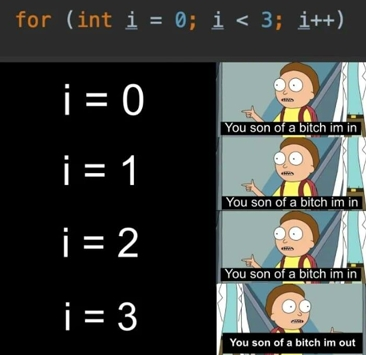
\includegraphics[width=0.5\linewidth]{cp4/loops.jpg}
    \end{figure}
\end{center}

% Basic
\section{Mayor}
Implemente un método que reciba un array de enteros y devuelva el mayor elemento del array.
\subsection*{Ejemplos}
\begin{itemize}
    \item Entrada: \( a = [3, 7, 2, 8, 4] \)\\
    Salida: \texttt{8}
    
    \item Entrada: \( a = [-5, -1, -10, -3] \)\\
    Salida: \texttt{-1}
    
    \item Entrada: \( a = [42] \)\\
    Salida: \texttt{42}
\end{itemize}

\section{Pertenece}
Implemente un método que reciba un array de enteros y devuelva si un número \(n\) pertenece al array \(a\).
\subsection*{Ejemplos}
\begin{itemize}
    \item Entrada: \( a = [3, 7, 2, 8, 4], \, n = 7 \)\\
    Salida: \textcolor{blue}{true} 
    
    \item Entrada: \( a = [3, 7, 2, 8, 4], \, n = 10 \)\\
    Salida: \textcolor{blue}{false}
    
    \item Entrada: \( a = [], \, n = 5 \)\\
    Salida: \textcolor{blue}{false}
\end{itemize}
 
\section{Índice}
Implemente un método que reciba un array de enteros y devuelva la posición (índice) de la primera aparición del número \(n\) en el array. Devuelve -1 si no aparece.
\subsection*{Ejemplos}
\begin{itemize}
   \item Entrada: \( a = [3, 7, 2, 8, 4], \, n = 8 \)\\
   Salida: \texttt{3}
   
   \item Entrada: \( a = [3, 7, 2, 8, 4], \, n = 10 \)\\
   Salida: \texttt{-1}
   
   \item Entrada: \( a = [5, 5, 5], \, n = 5 \)\\
   Salida: \texttt{0}
\end{itemize}
 
% Intermediate
\section{Segundo menor}
Implemente un método que reciba un array de números enteros y determine el segundo menor valor presente en el array. El método debe considerar únicamente valores distintos, si el array contiene menos de dos elementos únicos, debe lanzar una excepción indicando que no es posible determinar un segundo menor.
\subsection*{Ejemplos}
\begin{itemize}
    \item Entrada: \( \text{array} = [4, 1, 3, 2, 5] \)\\
    Salida: \textcolor{blue}{2}\\
    Explicación: Los elementos únicos ordenados son: \(1, 2, 3, 4, 5\).
    El segundo menor es \( 2 \).

    \item Entrada: \( \text{array} = [7, 7, 7, 7] \)\\
    Salida: \textcolor{red}{\texttt{Exception: No se puede determinar el segundo menor}}\\
    Explicación: El array solo tiene un valor único: \(7\).
    Se lanza una excepción porque no hay suficientes valores únicos.

    \item Entrada: \( \text{array} = [10, -3, -3, 0, 5] \)\\
    Salida: \textcolor{blue}{0}\\
    Explicación: Los elementos únicos ordenados son: \(-3, 0, 5, 10\).
    El segundo menor es \( 0 \).

    \item Entrada: \( \text{array} = [8] \)\\
    Salida: \textcolor{red}{\texttt{Exception: No se puede determinar el segundo menor}}\\
    Explicación: El array tiene un solo elemento. Se lanza una excepción porque no hay suficientes valores únicos.
\end{itemize}

\section{Promedio}
Implemente un método que reciba un array de enteros y devuelva: 
\begin{enumerate}
    \item El promedio de todos los elementos de un array.
    \item La cantidad de elementos que son mayor que el promedio en un array.
\end{enumerate}
\subsection*{Ejemplos}
\begin{itemize}
    \item Entrada: \( \text{array} = [4, 8, 6, 10, 2] \)\\
    Salida: 
    \begin{itemize}
        \item Promedio: 6.0.
        \item Elementos mayores que el promedio: 2.
    \end{itemize}
    Explicación: \(\frac{4 + 8 + 6 + 10 + 2}{5} = 6\).  
    Los elementos mayores que \( 6 \) son \( 8, 10 \), lo que da un total de \( 2 \).

    \item Entrada: \( \text{array} = [1, 1, 1, 1] \)\\
    Salida: 
    \begin{itemize}
        \item Promedio: 1.0.
        \item Elementos mayores que el promedio: 0.
    \end{itemize}
    Explicación: \(\frac{1 + 1 + 1 + 1}{4} = 1\).  
    No hay elementos mayores que \( 1 \), por lo que el resultado es \( 0 \).

    \item Entrada: \( \text{array} = [15, -5, 0, 10, 5] \)\\
    Salida: 
    \begin{itemize}
        \item Promedio: 5.0.
        \item Elementos mayores que el promedio: 2.
    \end{itemize}
    Explicación: \(\frac{15 + (-5) + 0 + 10 + 5}{5} = 5\).  
    Los elementos mayores que \( 5 \) son \( 15, 10 \), lo que da un total de \( 2 \).

    \item Entrada: \( \text{array} = [-10, -20, -30] \)\\
    Salida: 
    \begin{itemize}
        \item Promedio: -20.0.
        \item Elementos mayores que el promedio: 1.
    \end{itemize}
    Explicación: \(\frac{-10 + (-20) + (-30)}{3} = -20\).  
    El único elemento mayor que \( -20 \) es \( -10 \), por lo que el resultado es \( 1 \).
\end{itemize}

% Advanced
\section{Palíndromo}
\begin{enumerate}[label=\alph*)]
    \item Implemente un método que determine si el string \texttt{s} es un palíndromo, es decir, si se lee igual de izquierda a derecha que de derecha a izquierda.
    
    \begin{itemize}
        \item Entrada: \texttt{s = ana}\\
        Salida: \textcolor{blue}{true}

        \item Entrada: \texttt{s = anitalavalatina}\\
        Salida: \textcolor{blue}{true}

        \item Entrada: \texttt{s = palabra}\\
        Salida: \textcolor{blue}{false}
    \end{itemize}

    \item * Implemente un método que compute el menor string \texttt{t} tal que la concatenación de \texttt{s + t} forme un palíndromo.

    \begin{itemize}
        \item Entrada: \texttt{s = race}\\
        Salida: \texttt{car}\\
        Explicación: El string \texttt{''race''} no es un palíndromo. Para que la concatenación \texttt{s + t} sea un palíndromo, debemos agregar \texttt{''car''} al final, formando el palíndromo \texttt{''racecar''}.

        \item Entrada: \texttt{s = aba}\\
        Salida: \texttt{''''}\\
        Explicación: El string \texttt{''aba''} ya es palíndromo.

        \item Entrada: \texttt{s = anan}\\
        Salida: \texttt{a}\\
        Explicación: El string \texttt{''anan''} no es un palíndromo. Al agregar \texttt{''a''} al final, obtenemos el palíndromo \texttt{''anana''}.
    \end{itemize}
\end{enumerate}


\section{Mediana}
Sea \( A \) un array de enteros con \( n \) elementos (\( A = [a_1, a_2, \dots, a_n] \)), y supongamos que todos los elementos de \( A \) son \textbf{distintos}.

Definimos las cantidades de elementos menores y mayores con respecto a un valor \( m \) como:
\[
\text{menores}(m, A) = \lvert \{x \in A : x < m\} \rvert, \quad 
\text{mayores}(m, A) = \lvert \{x \in A : x > m\} \rvert.
\]

La \textbf{mediana} de \( A \) es un valor \( m \) que satisface las siguientes condiciones:

1. Si \( n \) es impar, la mediana es el elemento \( m \) tal que:
\[
\text{menores}(m, A) = \text{mayores}(m, A) = \frac{n}{2}.
\]

2. Si \( n \) es par, la mediana es el elemento \( m \) tal que:
\[
\text{menores}(m, A) = \frac{n}{2}, \quad 
\text{mayores}(m, A) = \frac{n}{2} - 1.
\]

Implemente un método que reciba un array de enteros distintos y devuelva el elemento mediana. 

\subsection*{Ejemplos:}
\begin{itemize}
    \item Entrada: \texttt{[3, 5, 2, 8, 1]}\\
    Salida: \texttt{3}\\
    Explicación: La cantidad de números menores que 3 (\texttt{[2, 1]}) es igual a la cantidad de números mayores que 3 (\texttt{[5, 8]}). Por lo tanto, la mediana es \texttt{3}.
    
    \item Entrada: \texttt{[3, 5, 2, 8]}\\
    Salida: \texttt{5}\\
    Explicación: En este caso, \texttt{5} tiene dos elementos menores (\texttt{[3, 2]}) y uno mayor (\texttt{[8]}). Por lo tanto, la mediana es \texttt{5}.
    
    \item Entrada: \texttt{[10, 3, 7, 5, 2]}\\
    Salida: \texttt{5}\\
    Explicación: El número \texttt{5} tiene la misma cantidad de elementos menores (\texttt{[2, 3]}) y mayores (\texttt{[7, 10]}). Por lo tanto, la mediana es \texttt{5}.
\end{itemize}

\section{Evaluando polinomios}
Sea \( p(x) \) un polinomio de grado \( n \) con coeficientes enteros, tal que:
    
\[
p(x) = a_n x^n + a_{n-1} x^{n-1} + \dots + a_1 x + a_0
\]

Este polinomio puede ser representado mediante un arreglo \( A = [a_0, a_1, \dots, a_n] \), donde el coeficiente \( a_k \) (con \( 0 \leq k \leq n \)) corresponde al término de grado \( k \). Así, el coeficiente de mayor grado se encuentra en la última posición del arreglo.

Por ejemplo:

\begin{itemize}
    \item El polinomio \( p(x) = 2x + 1 \) se representa como el arreglo \( A = [1, 2] \), donde \( a_0 = 1 \) y \( a_1 = 2 \).
    \item El polinomio \( p(x) = x^3 - 5x + 1 \) se representa como el arreglo \( A = [1, -5, 0, 1] \), donde \( a_0 = 1 \), \( a_1 = -5 \), \( a_2 = 0 \) y \( a_3 = 1 \).
\end{itemize}

Implemente un método que evalúe el valor del polinomio \( p(x) \) para un valor dado de \( x \). La evaluación del polinomio se realiza mediante la fórmula:

\[
p(x) = a_0 + a_1 x + a_2 x^2 + \dots + a_n x^n
\]

\textbf{Ejemplos:}
\begin{itemize}
    \item Entrada:
    \begin{itemize}
        \item Polinomio: \([1, 2]\) (representa \(p(x) = 2x + 1\))
        \item Valor de \(x\): \(3\)
    \end{itemize}
    Salida: \( p(3) = 7 \)
    
    \item Entrada:
    \begin{itemize}
        \item Polinomio: \([1, -5, 0, 1]\) (representa \(p(x) = x^3 - 5x + 1\))
        \item Valor de \(x\): \(2\)
    \end{itemize}
    Salida: \( p(2) = -1 \)
\end{itemize}

\section{Perímetro de un polígono}
Implemente un método que reciba un conjunto de \(n\) vértices de un polígono en el plano cartesiano, donde cada vértice está representado por un par de coordenadas \((x, y)\). Los vértices están ordenados y el último vértice se conecta con el primero, el método debe calcular y devolver el perímetro del polígono.
        
Sea \( P \) un polígono con \( n \) vértices, representados como un conjunto de pares ordenados de coordenadas en el plano cartesiano:
\[
P = \{ (x_1, y_1), (x_2, y_2), \dots, (x_n, y_n) \}
\]

donde \( (x_i, y_i) \) representa el \( i \)-ésimo vértice del polígono y los vértices están ordenados en el sentido en que se recorren los lados del polígono. 

El perímetro \( \text{Perímetro}(P) \) de un polígono es la suma de las longitudes de sus lados. Cada lado del polígono es la distancia euclidiana entre dos vértices consecutivos. Formalmente, la distancia entre dos vértices consecutivos \( (x_i, y_i) \) y \( (x_{i+1}, y_{i+1}) \) se calcula utilizando la fórmula de distancia euclidiana:

\[
d_i = \sqrt{(x_{i+1} - x_i)^2 + (y_{i+1} - y_i)^2}
\]

donde \( i = 1, 2, \dots, n-1 \), y se debe considerar también la distancia entre el último vértice \( (x_n, y_n) \) y el primer vértice \( (x_1, y_1) \), para cerrar el polígono:

\[
d_n = \sqrt{(x_1 - x_n)^2 + (y_1 - y_n)^2}
\]

Por lo tanto, el perímetro \( P \) del polígono es la suma de todas las distancias de los lados:

\[
\text{Perímetro}(P) = \sum_{i=1}^{n} d_i 
\]
\[
\text{Perímetro}(P) = \sum_{i=1}^{n-1} \sqrt{(x_{i+1} - x_i)^2 + (y_{i+1} - y_i)^2} + \sqrt{(x_1 - x_n)^2 + (y_1 - y_n)^2}
\]

\subsection*{Ejemplos}

\begin{itemize}
    \item Entrada: \([ (0, 0), (4, 0), (4, 3), (0, 3) ]\) \\
    Salida: 14.0
    \item Entrada: \([ (0, 0), (3, 0), (3, 3), (0, 3) ]\) \\
    Salida: 12.0
\end{itemize}